%% -*- coding: utf-8; -*-

\documentclass[
  master
  brazilian
]{ThesisPUC}


%%%
%%% Additional Packages
%%%

  \usepackage[brazilian]{babel}      %% in ThesisPUC.cls
  %% \usepackage[utf8]{inputenc}        %% .
  %% \usepackage[T1]{fontenc}           %% .
  %% \usepackage{lmodern}               %% .
  %% \usepackage[pdftex]{graphicx}	%% .

  \usepackage{tabularx}
  \usepackage{multirow}
  \usepackage{multicol}
  \usepackage{colortbl}
  \usepackage[%
    dvipsnames,
    svgnames,
    x11names,
    fixpdftex
  ]{xcolor}
  \usepackage{numprint}
  \usepackage{textcomp}
  \usepackage{booktabs}
  \usepackage{amsmath}
  \usepackage{enumitem}
  \usepackage{amssymb}
  \usepackage{textcomp}
% \usepackage{etoolbox}

%% numprint 
\npthousandsep{.}
\npdecimalsign{,}

%% ThesisPUC option
%\tablesmode{figtab} %% [nada, fig, tab ou figtab]
%\abreviationsmode{none} %% [none ou use] %% Default is [use]


%%%
%%% Counters
%%%

%% uncomment and change for other depth values
%% \setcounter{tocdepth}{3}
%% \setcounter{lofdepth}{3}
%% \setcounter{lotdepth}{3}
%% \setcounter{secnumdepth}{3}


%%%
%%% New commands and other global definitions
%%%

% -*- coding: iso-8859-1; -*-

%%%
%%% Newcommands
%%%

\newcommand{\degree}{\ensuremath{^\circ}}

\newcommand{\cetem}{Centro de Tecnologia Mineral}

\newcommand{\mybulletOB}{%
  % \textbullet
  % \checkmark
  $\triangleright$
  %\textopenbullet
}

\newcolumntype{L}{>{\raggedright \arraybackslash}X}
\newcolumntype{R}{>{\raggedleft \arraybackslash}X}
\newcolumntype{C}{>{\centering \arraybackslash}X}
\newcolumntype{M}[1]{>{\centering\hspace{0pt}}m{#1}}

\newcommand{\mrcel}[2]{%
\begin{tabular}[c]{@{}c@{}}#1\\#2\end{tabular}}

\newcommand{\mrcell}[2]{%
\begin{tabular}[l]{@{}l@{}}#1\\#2\end{tabular}}

\newcommand{\mrcelthree}[3]{%
\begin{tabular}[c]{@{}c@{}c@{}}#1\\#2\\#3\end{tabular}}

\newcommand{\mrcelcolorg}[2]{%
\begin{tabular}{l}\rowcolor{Gainsboro}#1\\#2\end{tabular}}

\newcommand{\mytbcimg}[3]{%
  \multicolumn{1}{C}{\parbox[c]{#1}{\includegraphics[width=#2]{#3}}}}


%%%
%%% Misc.
%%%

\usecolour{true}

%%%
%%% Titulos
%%%

\author{Julio César Álvarez Iglesias}
\authorR{Álvarez Iglesias, Julio César}

\advisor{Sidnei Paciornik}{Prof.}
\advisorR{Paciornik, Sidnei}
% If the advisor's department is different from author's department, uncomment the next line and type the correct name and acronym of advisor's institution.
%\advisorInst{institution name}{acronym}

\coadvisor{Otávio da Fonseca Martins Gomes}{Dr.}
\coadvisorR{da Fonseca Martins Gomes, Otávio}
\coadvisorInst{Centro de Tecnologia Mineral}{CETEM/MCTI}

%% \title{Desenvolvimento de um sistema de microscopia digital para
%%  classificação automática de tipos de hematita em minério de ferro}

\title{Desenvolvimento de um sistema de microscopia digital para
  classificação automática de tipos de hematita em minério de ferro}

\titleuk{Development of a digital microscopy system for automatic
  classification of hematite types in iron ore}

%% \subtitulo{Aqui vai o subtitulo caso precise}

\day{9}
\month{August}
\year{2012}

\city{Rio de Janeiro}
\CDD{620.11}
\department{Engenharia Química e de Materiais}
\program{Engenharia de Materiais e de Processos Químicos e Metalúrgicos}
\school{Centro Técnico Científico}
\university{Pontifícia Universidade Católica do Rio de Janeiro}
\uni{PUC-Rio}

%%%
%%% Jury
%%%

\jury{%
  \jurymember{Paulo Roberto Gomes Brandão}{Prof.}
    {Universidade Federal de Minas Gerais}{UFMG}
  \jurymember{Leonardo Evangelista Lagoeiro}{Prof.}
    {Universidade Federal de Ouro Preto}{UFOP}
  \jurymember{Reiner Neumann}{Dr.}
    {Centro de Tecnologia Mineral}{CETEM/MCTI}
  \jurymember{Marcos Henrique de Pinho Maurício}{Dr.}
    {Departamento de Engenharia Química e de Materiais}{PUC-Rio}
}

%%%
%%% Resume
%%%

\resume{%
  Majored in physics by the University of Havana (Havana,
  Cuba)...}

%%%
%%% Acknowledgment (REMINDER TO SCHOLARSHIP STUDENTS. Do not forget to thank the agencies that supported your work.)
%%%

\acknowledgment{%
  \noindent I would like to first thank my advisor ...
  \bigskip

  \noindent Then I wish to thank ...
}

%%%
%%% Catalog prekeywords
%%%

\catalogprekeywords{%
  \catalogprekey{Engenharia Química}%
  \catalogprekey{Engenharia de Materiais}%
}

%%%
%%% Keywords
%%%

\keywords{%
  \key{Minério de Ferro}
  \key{Cristais de Hematita}
  \key{Microscopia Digital}
  \key{Análise de Imagens}
  \key{Classificação}
  \key{Microscopia de Luz Polarizada}
}

\keywordsuk{%
  \key{Iron Ore}%
  \key{Hematite Crystals}%
  \key{Digital Microscopy}%
  \key{Image Analysis}%
  \key{Classification}%
  \key{Polarized Light Microscopy}%
}

%%%
%%% Abstract
%%%

\abstract{%
  O minério de ferro é um material policristalino oriundo de processos
  naturais complexos durante tempos geológicos, que dão origem ...
}

\abstractuk{%
  Iron ore is a polycrystalline material created by complex natural
  processes during geological periods, which give rise to ...}

%%%
%%% Dedication
%%%

\dedication{%
  To my parents, for their support\\
and encouragement.
}

%%%
%%% Epigraph
%%%

\epigraph{%
  My beautifull epigraph
}
\epigraphauthor{Wassily Kandinsky}
\epigraphbook{Regards sur le passé}

%%%
%%% Hyphenation
%%%

\hyphenation{PON-TI-FÍ-CIA}

%%%
%%% 
%%%

\begin{document}

  % -*- coding: utf-8; -*-

\chapter{Introduction}

This is the first chapter...

In this chapter, let's have a nice image:

\begin{figure} [h]
  \begin{center}
    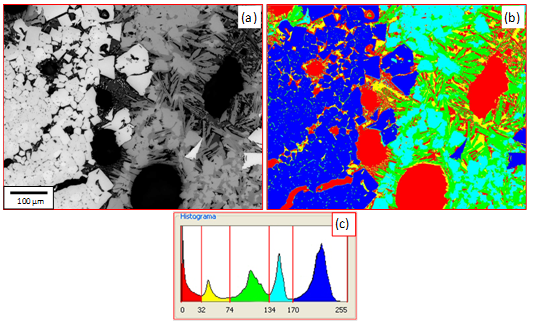
\includegraphics[height=243pt,width=400pt]{images/fig2-6}
    \caption{Example of thresholding: (a) original image; (b) processed
      image.\cite{74}}\label{fig:2-6}
  \end{center}
\end{figure}

  % -*- coding: utf-8; -*-

\chapter{Review}

This is the second chapter...

In this chapter, let's have a nice table:

%% -*- coding: utf-8; -*-

\begin{table} [!h]
  \caption{Principais minerais de ferro e suas classes.\cite{29}}\label{tab:2-4}
  ~\\[-1mm]
   \begin{tabularx}
     {\textwidth}
     { p{2.0cm}
       p{2.5cm}
       p{3.3cm}
       p{1.3cm}
       p{2.7cm}}

     \textbf{Classes}
     & \textbf{Minerais}
     & \textbf{\mrcel {Fórmula}{Química}}
     & \textbf{\mrcel{Teor}{de Fe}}
     & \textbf{\mrcel{~~Designação}{~~Comum}}
     \\\toprule

     ~ \\[-6mm]
     \multirow{5}{*}{Óxidos}& Magnetita
     & $Fe_{3}O_{4}$
     & ~72,4
     & \mrcel{~~Óxido ferroso}{~~férrico}
     \\%\midrule

     & Hematita
     & $Fe_{2}O_{3}$
     & ~69,9
     & ~~Óxido férrico \\[2mm]

     & Goethita
     & $FeO(OH)$
     & ~62,8
     & \multirow{2}{*}{\mrcel{Óxido-hidróxido}{de ferro}} \\[2mm]


     & Lepidocrocita
     & $FeO(OH)$
     & ~62,8 &
     \\\midrule

     Carbonato
     & Siderita
     & $FeCO_{3}$
     & ~48,2
     & \mrcel{~~~~Carbonato}{~~~~de Ferro}
     \\\midrule

     \multirow{2}{*}{Sulfetos}
     & Pirita
     & $FeS_{2}$
     & ~46,5
     & \multirow{2}{*}{~} \\[2mm]


     & Pirrotita
     & $FeS$
     & ~63,6
     & ~
     \\\midrule

     \multirow{10}{*}{Silicatos}
     & Fayalita
     & $Fe^{2+}_{2}(SiO_{4})$
     & ~54,8
     & \mrcel{~~~~Grupo da}{~~~~Olivina} \\[4mm]

     & Laihunite
     & $Fe^{2+}Fe^{3+}_{2}(SiO_{4})_{2}$
     & ~47,6
     & \mrcel{~~~~Grupo da}{~~~~Olivina} \\[4mm]

     & Greenalita
     & \mrcell{$2Fe^{2+}_{2}6Fe^{3+}Si_{2}$}{$4O_{5}(OH)_{3,3}$}
     & ~44,1
     & \mrcel{~~~~Grupo da}{~~~~Serpentina} \\[4mm]

     & Grunerita
     & \mrcell{$Fe^{2+}_{7}(Si_{8}O_{22})$}{$(OH)_{2}$}
     & ~39,0
     & \mrcel{~~~~Grupo dos}{~~~~Anfibólios} \\[4mm]

     & Fé-antofilita
     & \mrcell{$Fe^{2+}_{7}(Si_{8}O_{22})$}{$(OH)_{2}$}
     & ~39,0
     & \mrcel{~~~~Grupo dos}{~~~~Anfibólios}
     \\\midrule
   \end{tabularx}
\end{table}

% -*- coding: utf-8; -*-

\newcommand{\coltworowone}{%
\begin{tabular}{ l @{\extracolsep{2mm}}X }
  \mybulletOB
    & Cristais ~~ muito	\\[-1.2mm]
  ~ & pequenos, 	\\[-.4mm]
  ~ & $<0.01$ mm. \\
  \mybulletOB & Textura porosa. \\
  \mybulletOB
    & Contatos pouco	\\[-1.2mm]
  ~ & desenvolvidos.
\end{tabular}}

\newcommand{\coltworowtwo}{%
\begin{tabular}{ l @{\extracolsep{2mm}}X }
  \mybulletOB
    & Cristais euédricos \\[-1.2mm]
  ~ & isolados ~ ou ~ em \\[-1.2mm]
  ~ & agregados. \\
  \mybulletOB
    & Cristais compac- \\[-1.2mm]
  ~ & tos.
\end{tabular}}

\newcommand{\coltworowthree}{%
\begin{tabular}{ l @{\extracolsep{2mm}}X }
  \mybulletOB
    & Hematita ~~ com \\[-1.2mm]
  ~ & hábito de magne- \\[-1.2mm]
  ~ & tita. \\
  \mybulletOB
    & Oxidação segundo \\[-1.2mm]
  ~ & os planos ~ crista- \\[-1.2mm]
  ~ & lográficos da mag- \\[-1.2mm]
  ~ & netita. \\
  \mybulletOB
    & Geralmente ~ po- \\[-1.6mm]
  ~ & rosa.
\end{tabular}}

\newcommand{\coltworowfour}{%
\begin{tabular}{ l @{\extracolsep{2mm}}X }
  \mybulletOB
    & Formatos irregu- \\[-1.2mm]
  ~ & lares ~~ inequidi- \\[-1.2mm]
  ~ & mensionais. \\
  \mybulletOB
    & Contatos irregula-\\[-1.2mm]
  ~ & res, ~ geralmente \\[-1.2mm]
  ~ & imbricados.
 \end{tabular}}

\newcommand{\coltworowfive}{%
\begin{tabular}{ l @{\extracolsep{2mm}}X }
  \mybulletOB
    & Formatos regula- \\[-1.2mm]
  ~ & res ~~ equidimen- \\[-1.2mm]
  ~ & sionais. \\
  \mybulletOB
    & Contatos ~~ retilí- \\[-1.2mm]
  ~ & neos ~ e ~ junções \\[-1.2mm]
  ~ & tríplices. \\
  \mybulletOB
    & Cristais compac-\\[-1.6mm]
  ~ & tos.
 \end{tabular}}

\newcommand{\coltworowsix}{%
\begin{tabular}{ l @{\extracolsep{2mm}}X }
  \mybulletOB
    & Cristais inequidi- \\[-1.2mm]
  ~ & mensionais, hábi- \\[-1.2mm]
  ~ & to tabular. \\
  \mybulletOB
    & Contato retilíneo. \\
  \mybulletOB
    & Cristais compac- \\[-1.6mm]
  ~ & tos.
 \end{tabular}}

\newcommand{\coltworowseven}{%
\begin{tabular}{ l @{\extracolsep{2mm}}X }
  \mybulletOB
    & Material cripto- \\[-1.2mm]
  ~ & cristalino.  \\
  \mybulletOB
    & Estrutura colofor- \\[-1.2mm]
  ~ & me, hábito botri- \\[-1.2mm]
  ~ & oidal.  \\
  \mybulletOB
    & Textura porosa.
 \end{tabular}}

\begin{table} [!p]
    \caption{Main morphologies of hematite.\cite{14}}\label{tab:2-5}
    ~\\[-2mm]
  \begin{tabularx}{\textwidth}{@{\extracolsep{0pt}}C @{\extracolsep{0pt}}C C C}

    \textbf{Tipo}
    & \textbf{Características}
    & \textbf{\mrcel{Forma}{Textura}}
    & \textbf{\mrcel{Ilustração}{Esquemática}}
    \\\toprule

    ~ \\[-6mm]
    \mrcel{Hematita}{Microcristalina}
    & \coltworowone
    & \mytbcimg{2.3cm}{2.9cm}{images/Microcristalina}
    & \mytbcimg{2.6cm}{2.5cm}{images/MicrocristalinaEsq}
    \\\midrule

    ~\\[-6mm]
    Magnetita
    & \coltworowtwo
    & \mytbcimg{2.3cm}{2.9cm}{images/Magnetita}
    & \mytbcimg{2.6cm}{2.9cm}{images/MagnetitaEsq}
    \\\midrule

    ~\\[-5mm]
    Martita
    & \coltworowthree
    & \mytbcimg{2.3cm}{2.9cm}{images/Martita}
    & \mytbcimg{2.6cm}{2.9cm}{images/MartitaEsq}
    \\\midrule

    ~\\[-5mm]
    \mrcel{Hematita}{Lobular}
    & \coltworowfour
    & \mytbcimg{2.3cm}{2.9cm}{images/Lobular}
    & \mytbcimg{2.6cm}{2.9cm}{images/LobularEsq}
    \\\midrule

    ~\\[-5mm]
    \mrcel{Hematita}{Granular}
    & \coltworowfive
    & \mytbcimg{2.3cm}{2.9cm}{images/Granular}
    & \mytbcimg{2.6cm}{2.9cm}{images/GranularEsq}
    \\\midrule

    ~\\[-5mm]
    \mrcel{Hematita}{Lamelar}
    & \coltworowsix
    & \mytbcimg{2.3cm}{2.9cm}{images/Lamelar}
    & \mytbcimg{2.6cm}{2.9cm}{images/LamelarEsq}
    \\\midrule

    ~\\[-5mm]
    \mrcelthree{Hidróxidos de}{ Fe (Goethita-}{Limonita)}
    & \coltworowseven
    & \mytbcimg{2.3cm}{2.9cm}{images/Goethita}
    & \mytbcimg{2.6cm}{2.9cm}{images/GoethitaEsq}
    \\\midrule

  \end{tabularx}
\end{table}


\section{Hematite}

A hematita é o mineral de ferro mais importante devido a sua alta
ocorrência em vários tipos de rochas e suas origens diversas.\cite{30}
A composição química deste mineral é Fe$_{2}$O$_{3}$, com uma fração
mássica em ferro de 69,9\% e uma fração mássica em oxigênio de
30,1\%.\cite{31}

...


\subsection{Martite}

A hematita é o mineral de ferro mais importante devido a sua alta
ocorrência em vários tipos de rochas e suas origens diversas.\cite{30}
A composição química deste mineral é Fe$_{2}$O$_{3}$, com uma fração
mássica em ferro de 69,9\% e uma fração mássica em oxigênio de
30,1\%.\cite{31}

...


\subsubsection{Globular}

A hematita é o mineral de ferro mais importante devido a sua alta
ocorrência em vários tipos de rochas e suas origens diversas.\cite{30}
A composição química deste mineral é Fe$_{2}$O$_{3}$, com uma fração
mássica em ferro de 69,9\% e uma fração mássica em oxigênio de
30,1\%.\cite{31}

...

\subsubsection{Escaping percent in a title:  100\%}

  % -*- coding: utf-8; -*-

\chapter{Conclusão}

Assim, como uma proposta para trabalho futuro, pode-se buscar combinar
os dois enfoques...

  %% ...
  \arial
  \bibliography{tiny}
  \normalfont
  % -*- coding: utf-8; -*-

\appendix
\chapter{Published paper}

The following paper was published ...

\end{document}
